\subsubsection{Regge Theory}
Regge theory can be used to  describe the production of the \piz meson in photoproduction. According to Regge theory the reaction amplitudes can be described by Regge poles in which the dominant Regge poles originate from t-channel exchange. This model has been developed over the years and is greatly described in~\cite{JPAC}. Using this model along with the \g12 measurements, seen in figure~\ref{fig:pi0_regge}, it is shown that this theory provides a good description of the data obtained by \g12 and a previous measurement~\cite{brem}.
\begin{figure}[h]
	\centerline{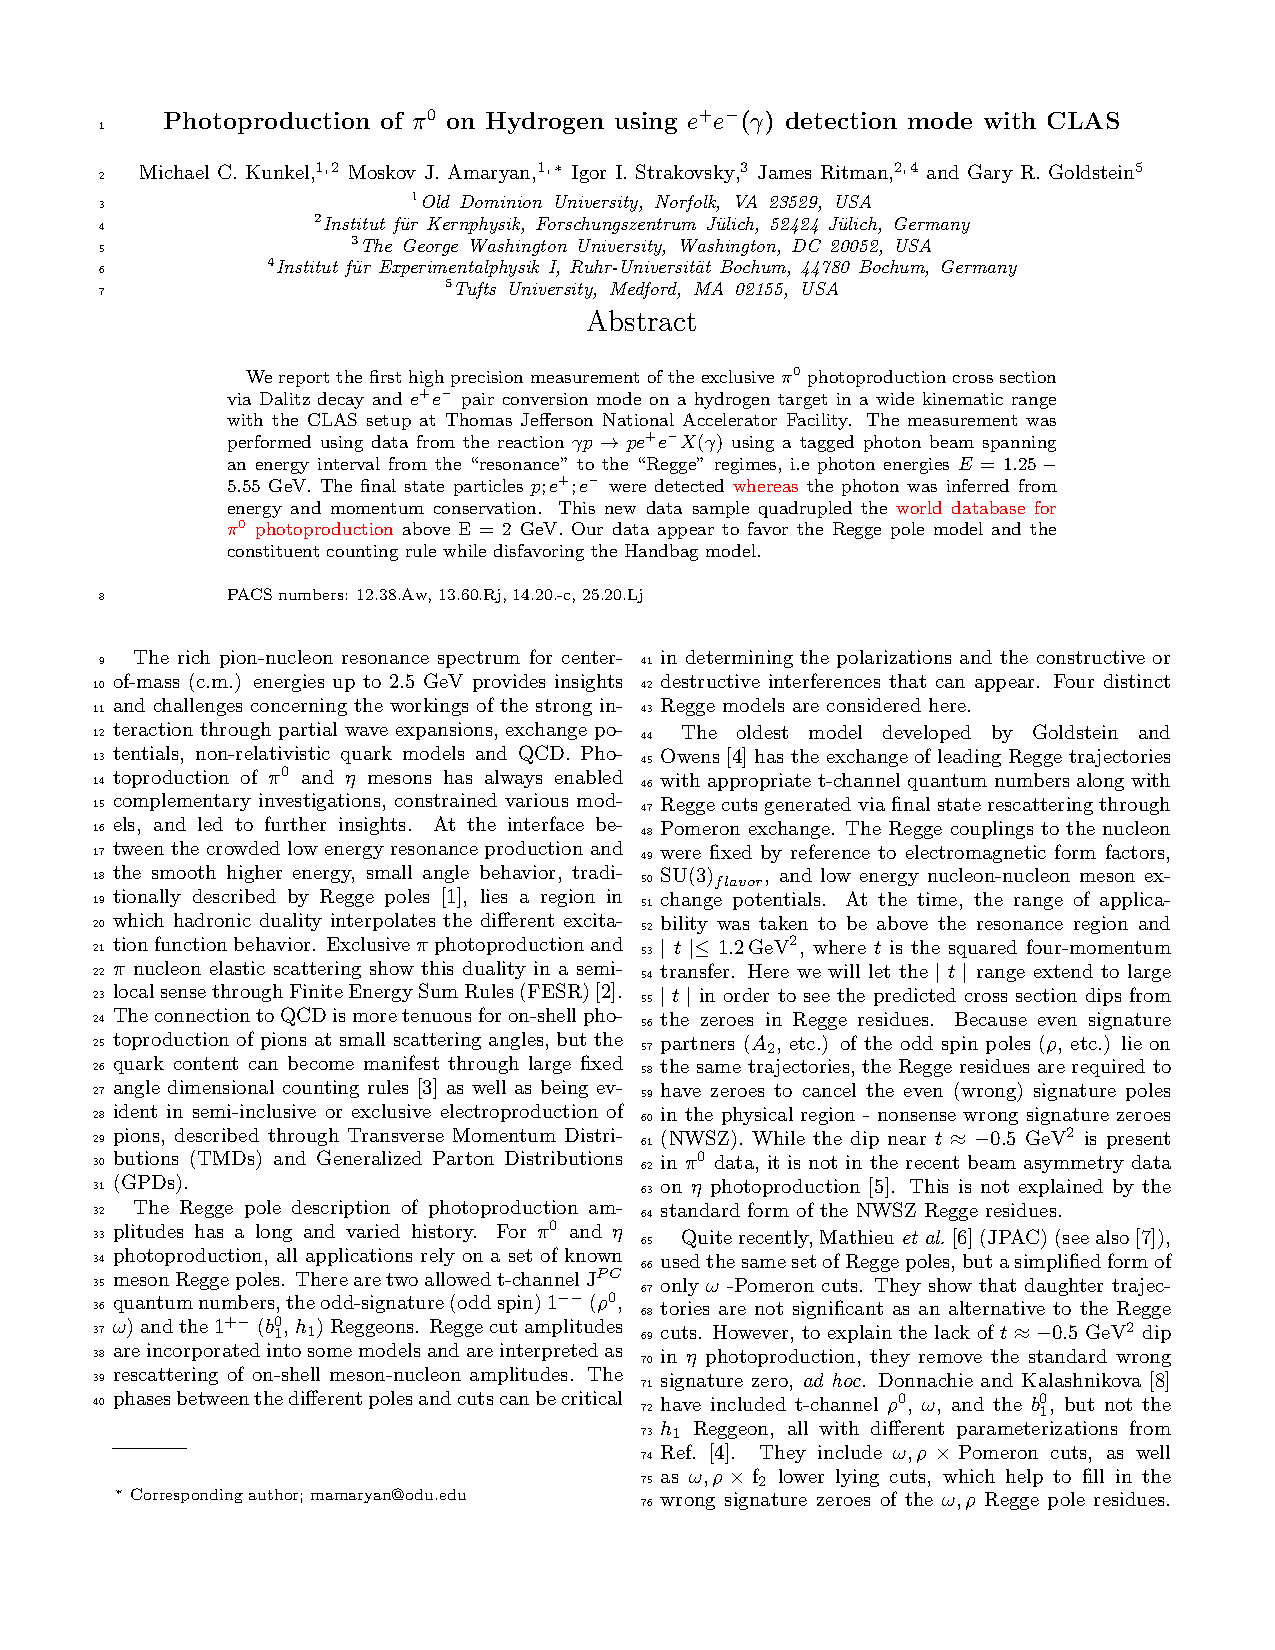
\includegraphics[width=275 pt, height = 160 pt]{\figures/analysis/DSG/pi0_regge.pdf}}
	\caption{Comparison with Regge model. Experimental data are from the current measurement (red filled circles) and previous bremsstrahlung measurements~\protect\cite{brem} (black open circles). }
	\label{fig:pi0_regge}
\end{figure}